\section{Three-Class Classification}
\lb{sec:3class}

One of the caveats of the analysis with two classes is that there are associated sources, which do not belong to AGN or PSR classes. These have the labels: unk, spp, glc, snr, gal, sbg, GAL, sfr, bin, SNR, HMB, LMB, css, PWN, pwn, hmb, SFR, BIN, lmb, NOV.
We collect all these associated sources, which do not belong to AGN and PSR classes into a new class, which we label as ``OTHER''.
Since in two-class classification we train algorithm to classify sources only into AGN and PSR classes, OTHER sources are also classified as either AGN or PSR.
This introduces a bias in the estimates of the number of AGNs and pulsars among unassociated sources.
One possibility to correct this bias is to assume that the fractions of OTHER sources among associated and unassociated sources are the same (Equation (\ref{eq:other_correction})).
This correction can be applied for the total number of sources or for the number of sources in some window of parameters,
e.g., in a flux bin or in a range of latitudes and longitudes.
This is a straightforward calculation but it has some limitations. In particular, it implicitly assigns equal probabilities to all AGNs (and all PSRs) to belong to the OTHER class.
For a small range of parameters the variance of this estimate can be very large due to small number of associated OTHER sources in this parameter range.
As we will see in Section \ref{sec:pop_studies}, this correction depends on the choice of the variable used for binning, e.g.,
overall correction with latitude bins is not equal to the correction with longitude bins.

In this section we discuss the construction of probabilistic catalogs with multi-class classification (3-class classification in our case).
We start with the construction of the probabilistic catalog based on 3FGL by adding the class ``OTHER'', which includes all associated sources without AGN or PSR associations: there are 108 such sources in 3FGL.
We use the same 11 features as in the 2-class classification: the only difference is that we use cos(GLON) instead of GLON.
The reason is that LR and NN methods have a significantly worse performance than RF and BDT methods when we use GLON,
but, as we show below, all four methods have comparable accuracy when we use cos(GLON).
This can be due to discontinuity in the GLON variable. 
We perform optimization of the meta-parameters for the four ML algorithms with the 3 classes.


\begin{figure}[h]
\center
%\hspace*{-1cm}
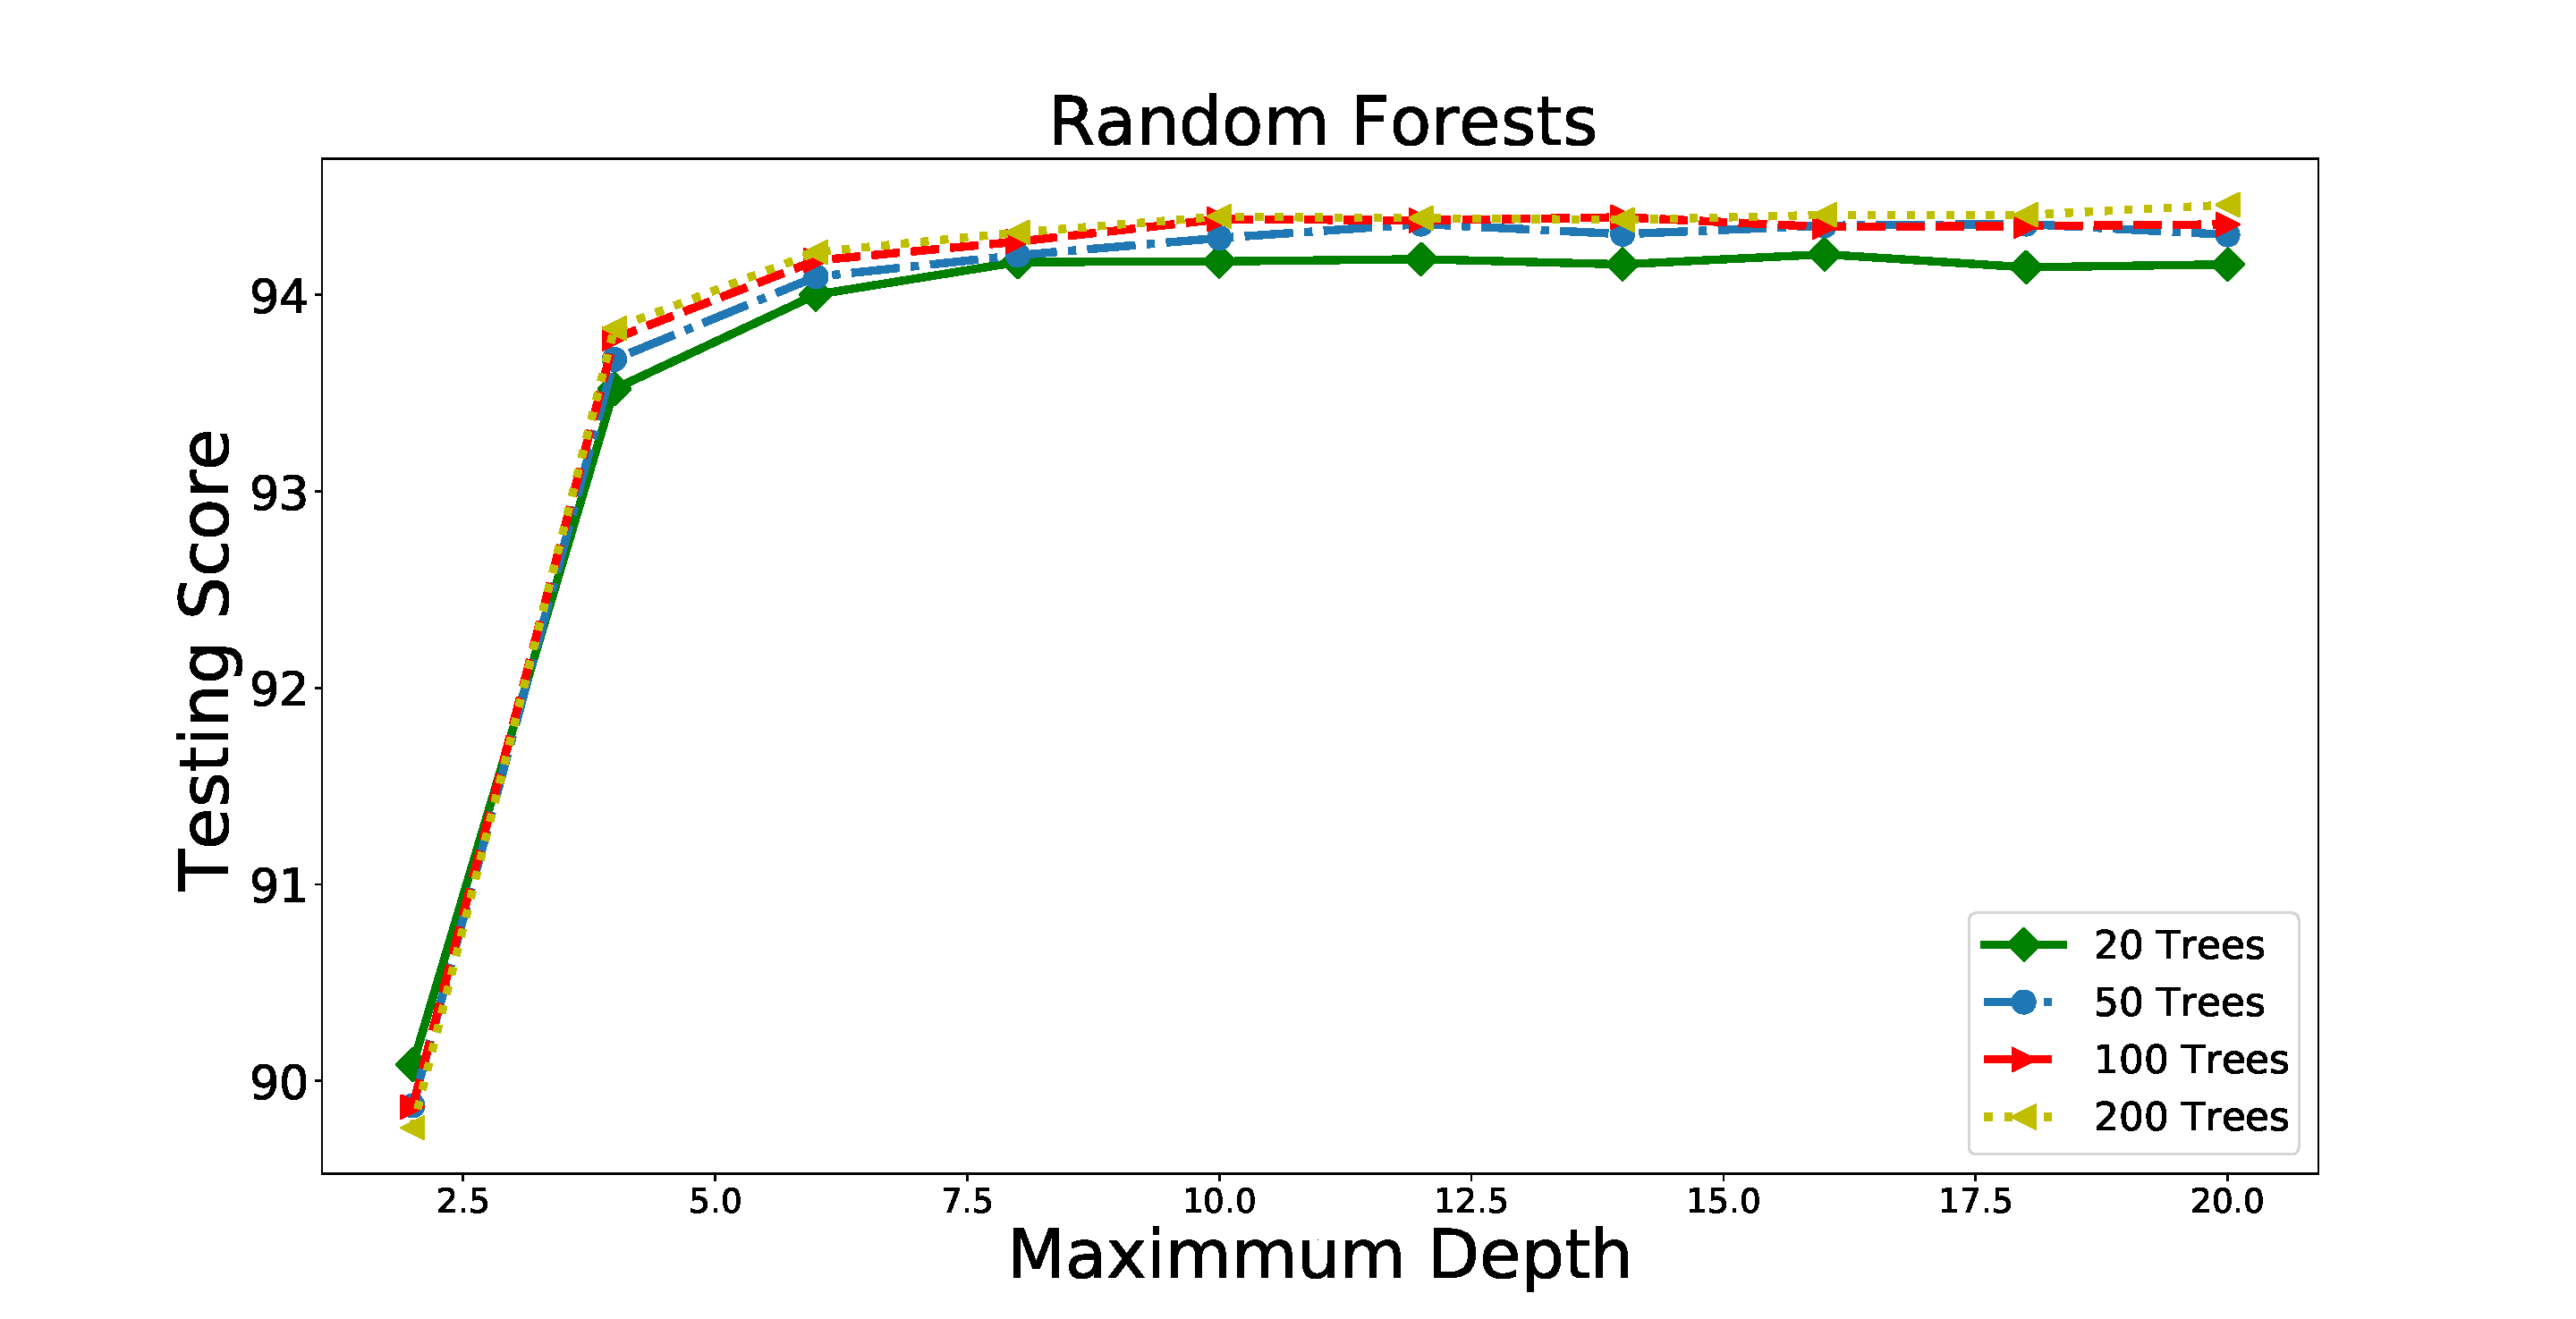
\includegraphics[width=0.5\textwidth]{plots/rf_train_multi.pdf}\\
%\hspace*{-1cm}
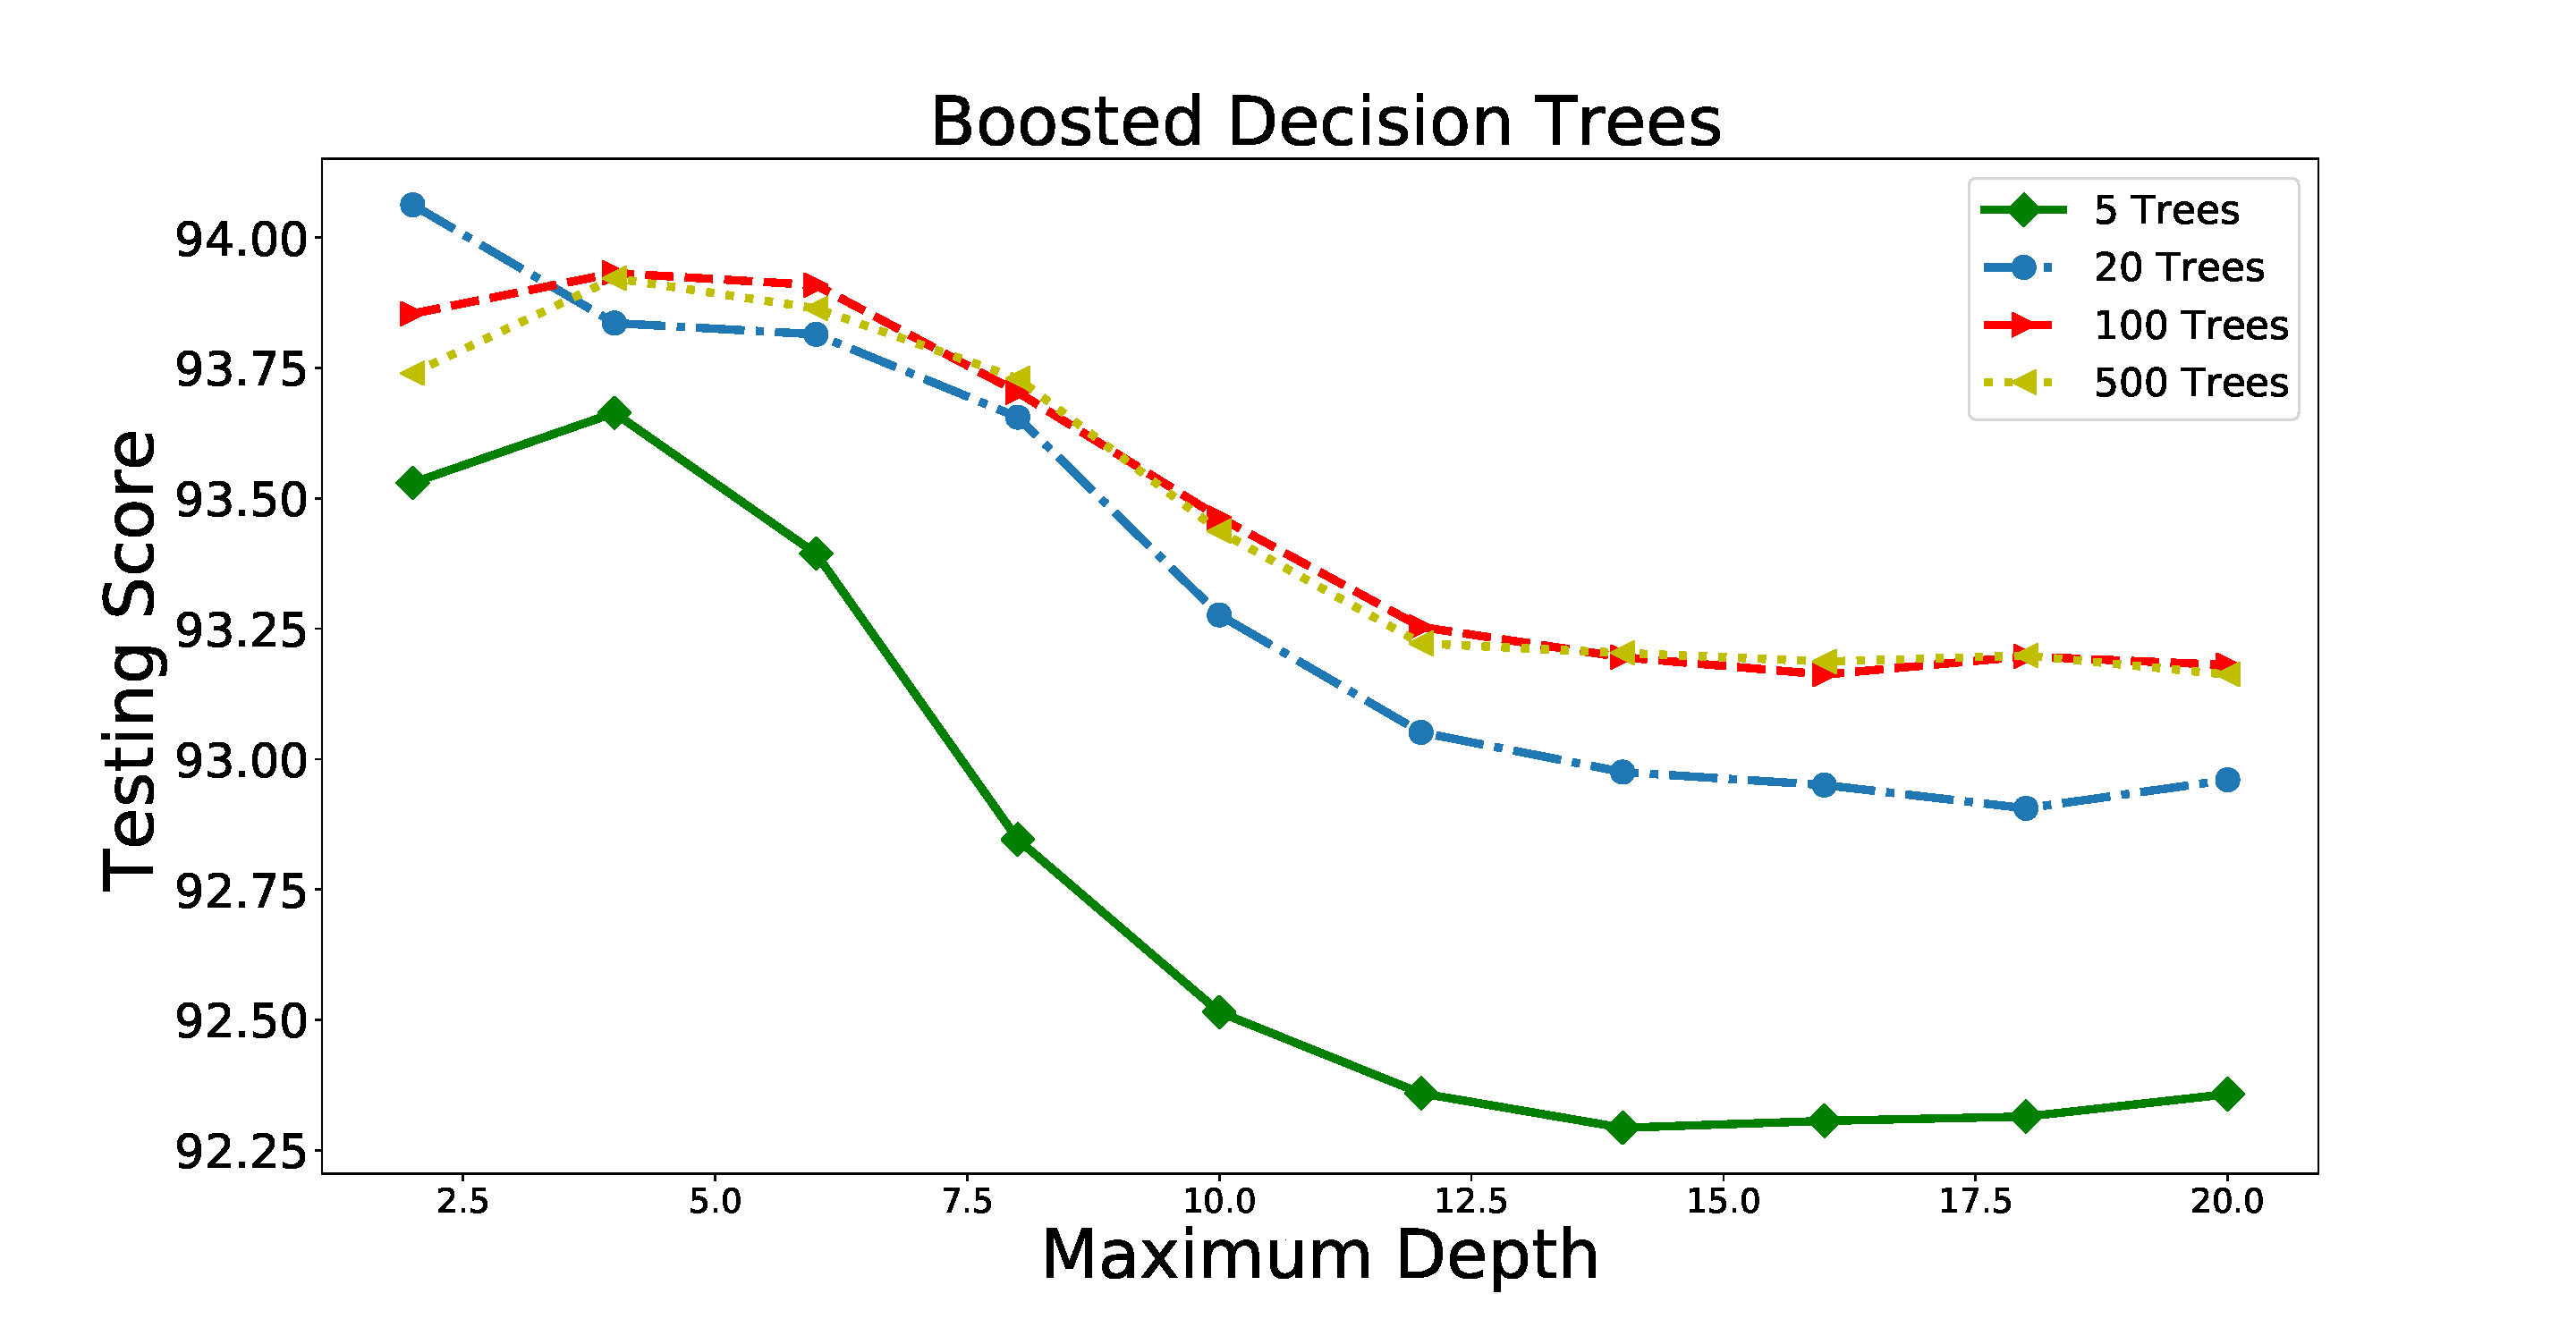
\includegraphics[width=0.5\textwidth]{plots/bdt_train_multi.pdf}
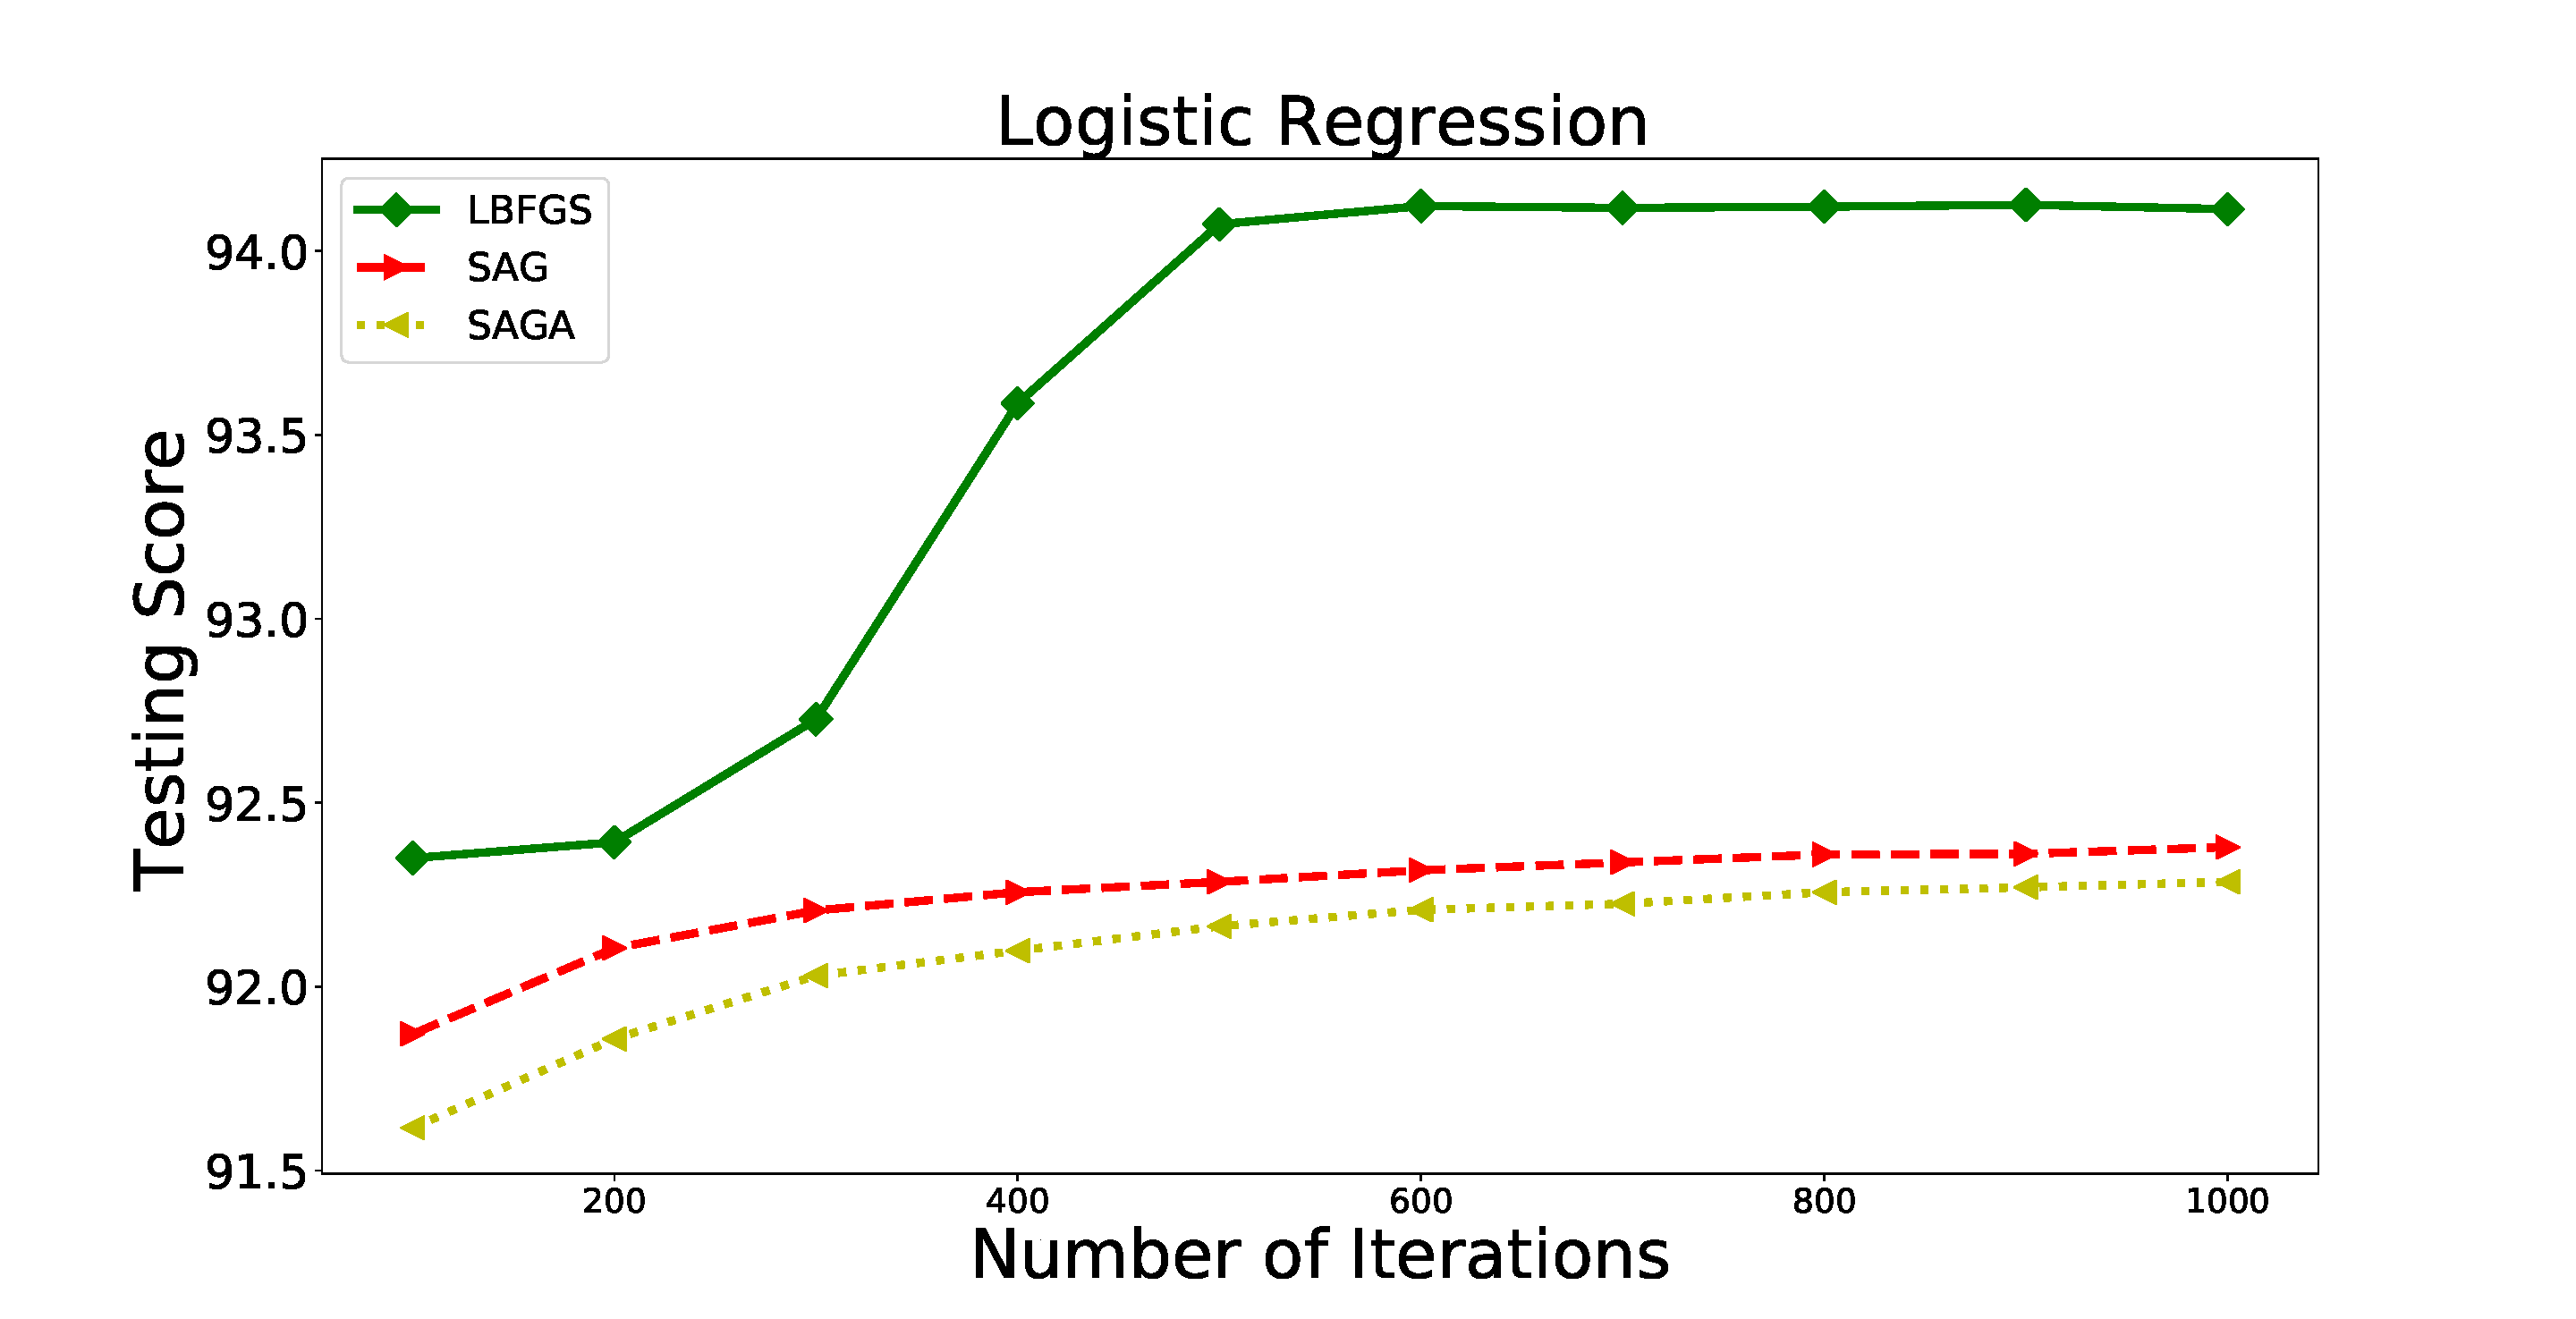
\includegraphics[width=0.5\textwidth]{plots/lr_train_multi.pdf}
\caption{Accuracy for the 3-class classification with RF, BDT and LR  methods. LR does not have liblinear solver here, since liblinear cannot handle multinomial loss.
}
\label{fig:tree_multi}
\end{figure}

\begin{figure}[h]
\center
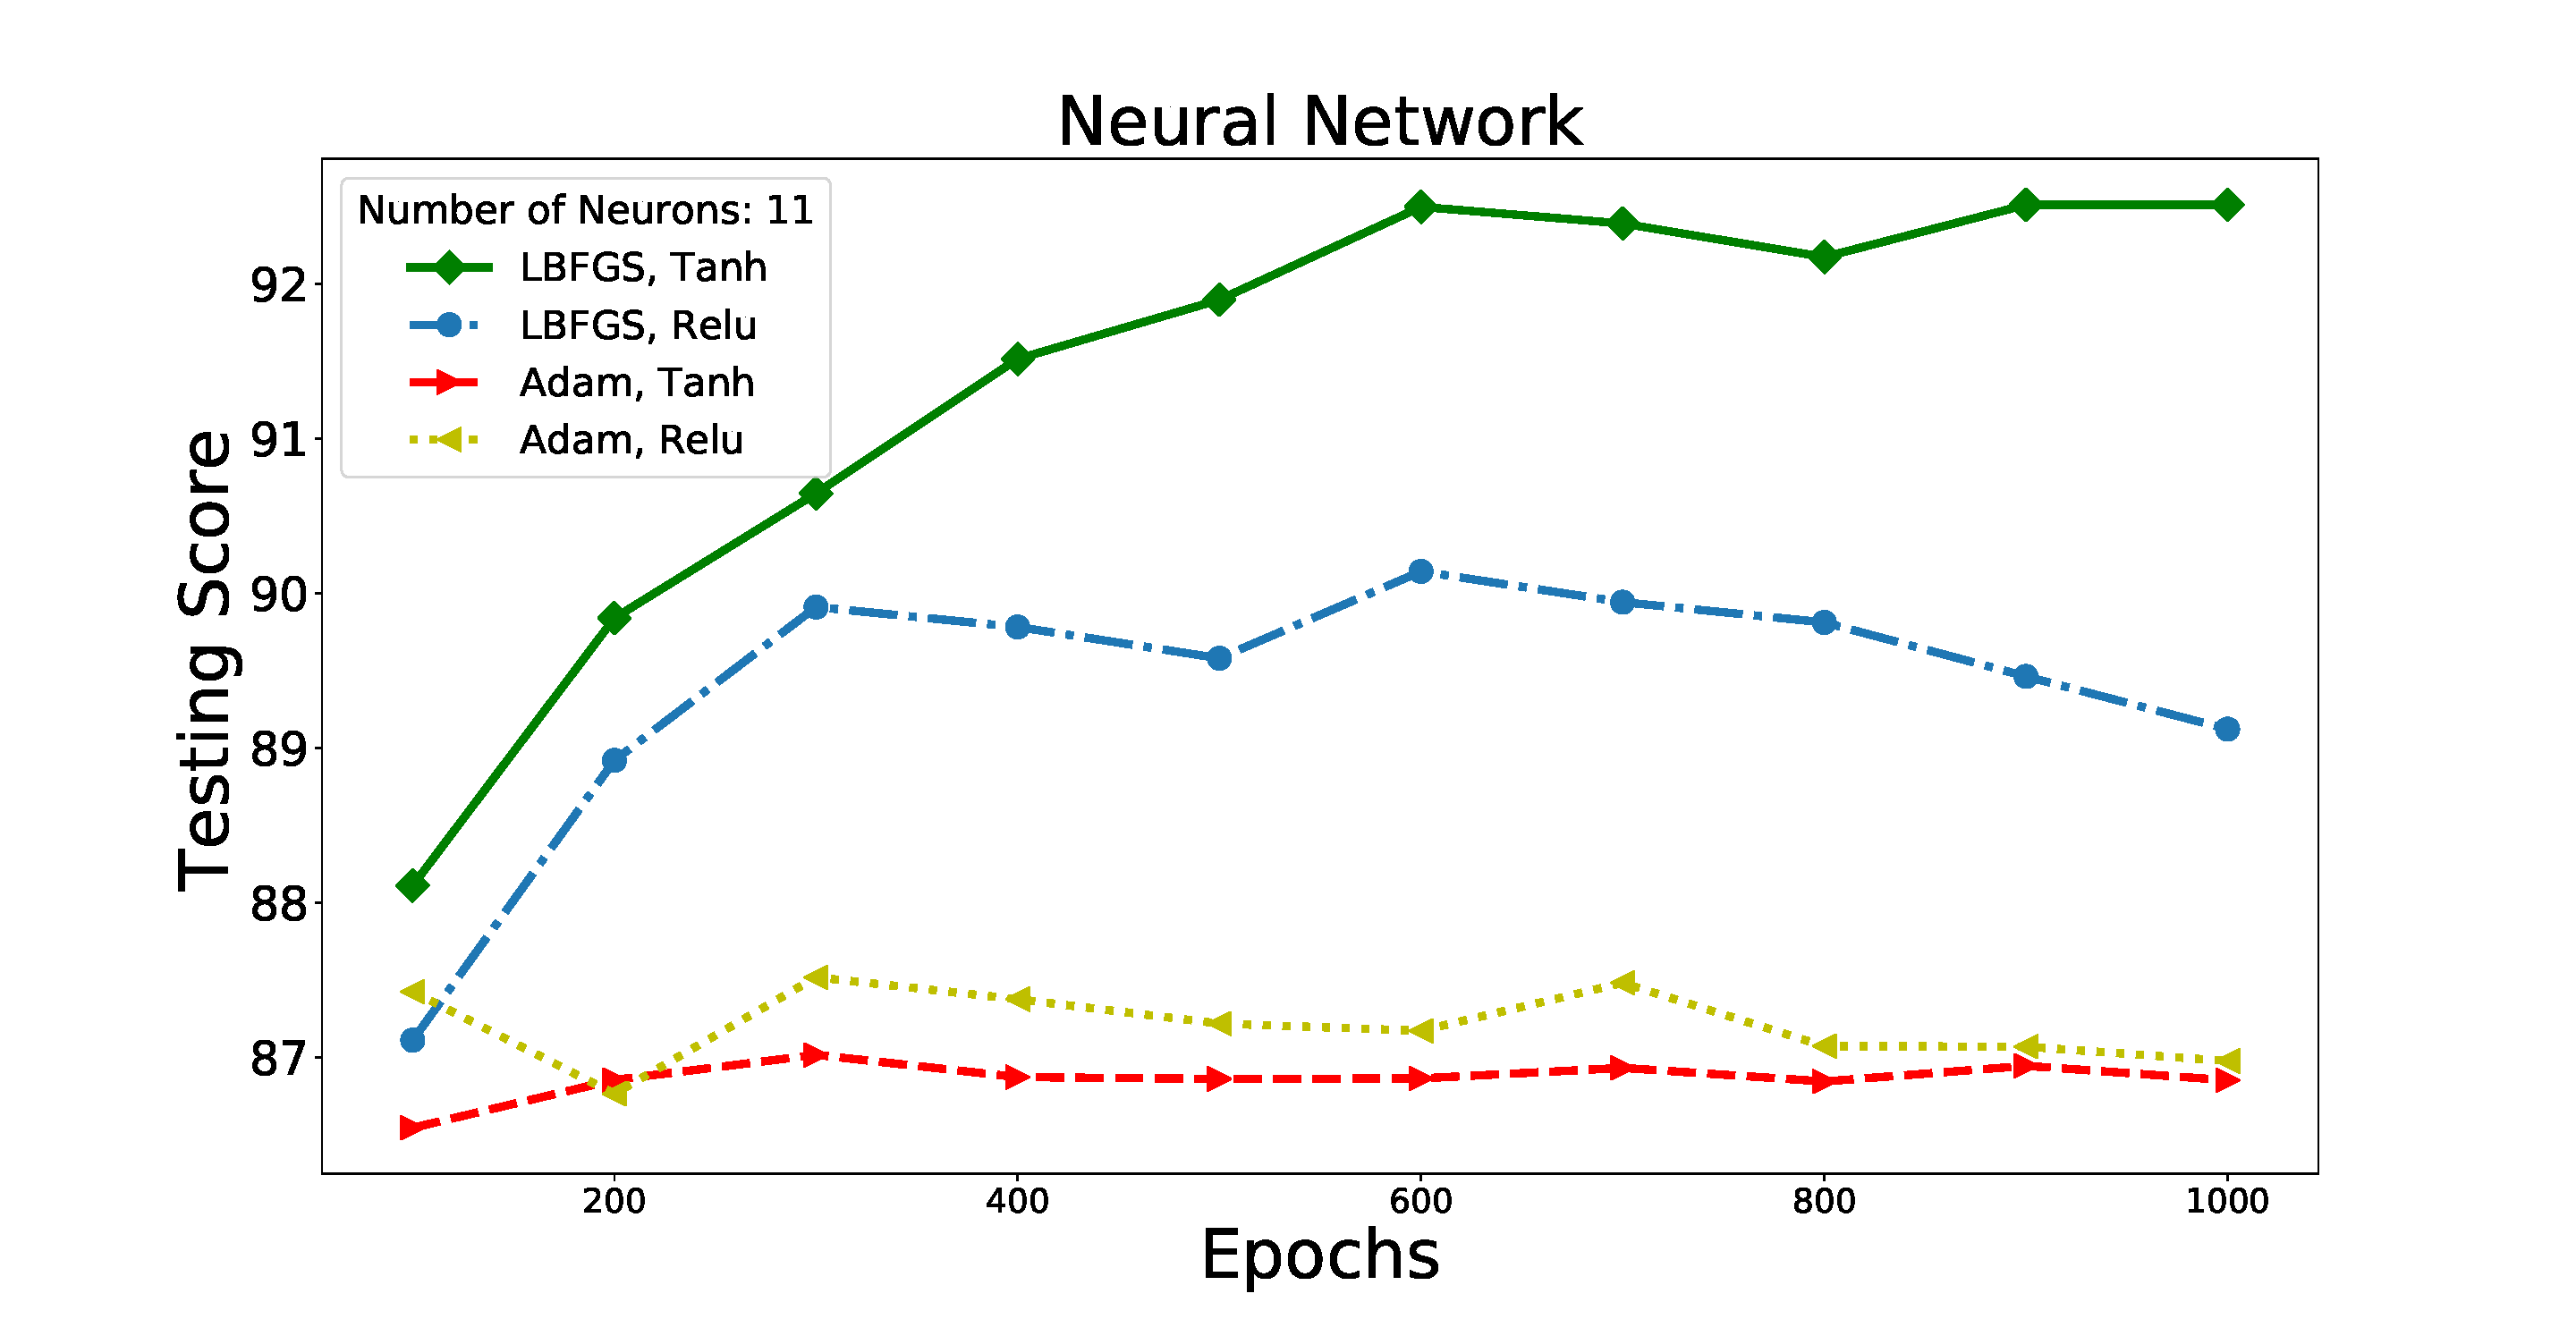
\includegraphics[width=0.5\textwidth]{plots/nn_epoch_train_multi.pdf}\\
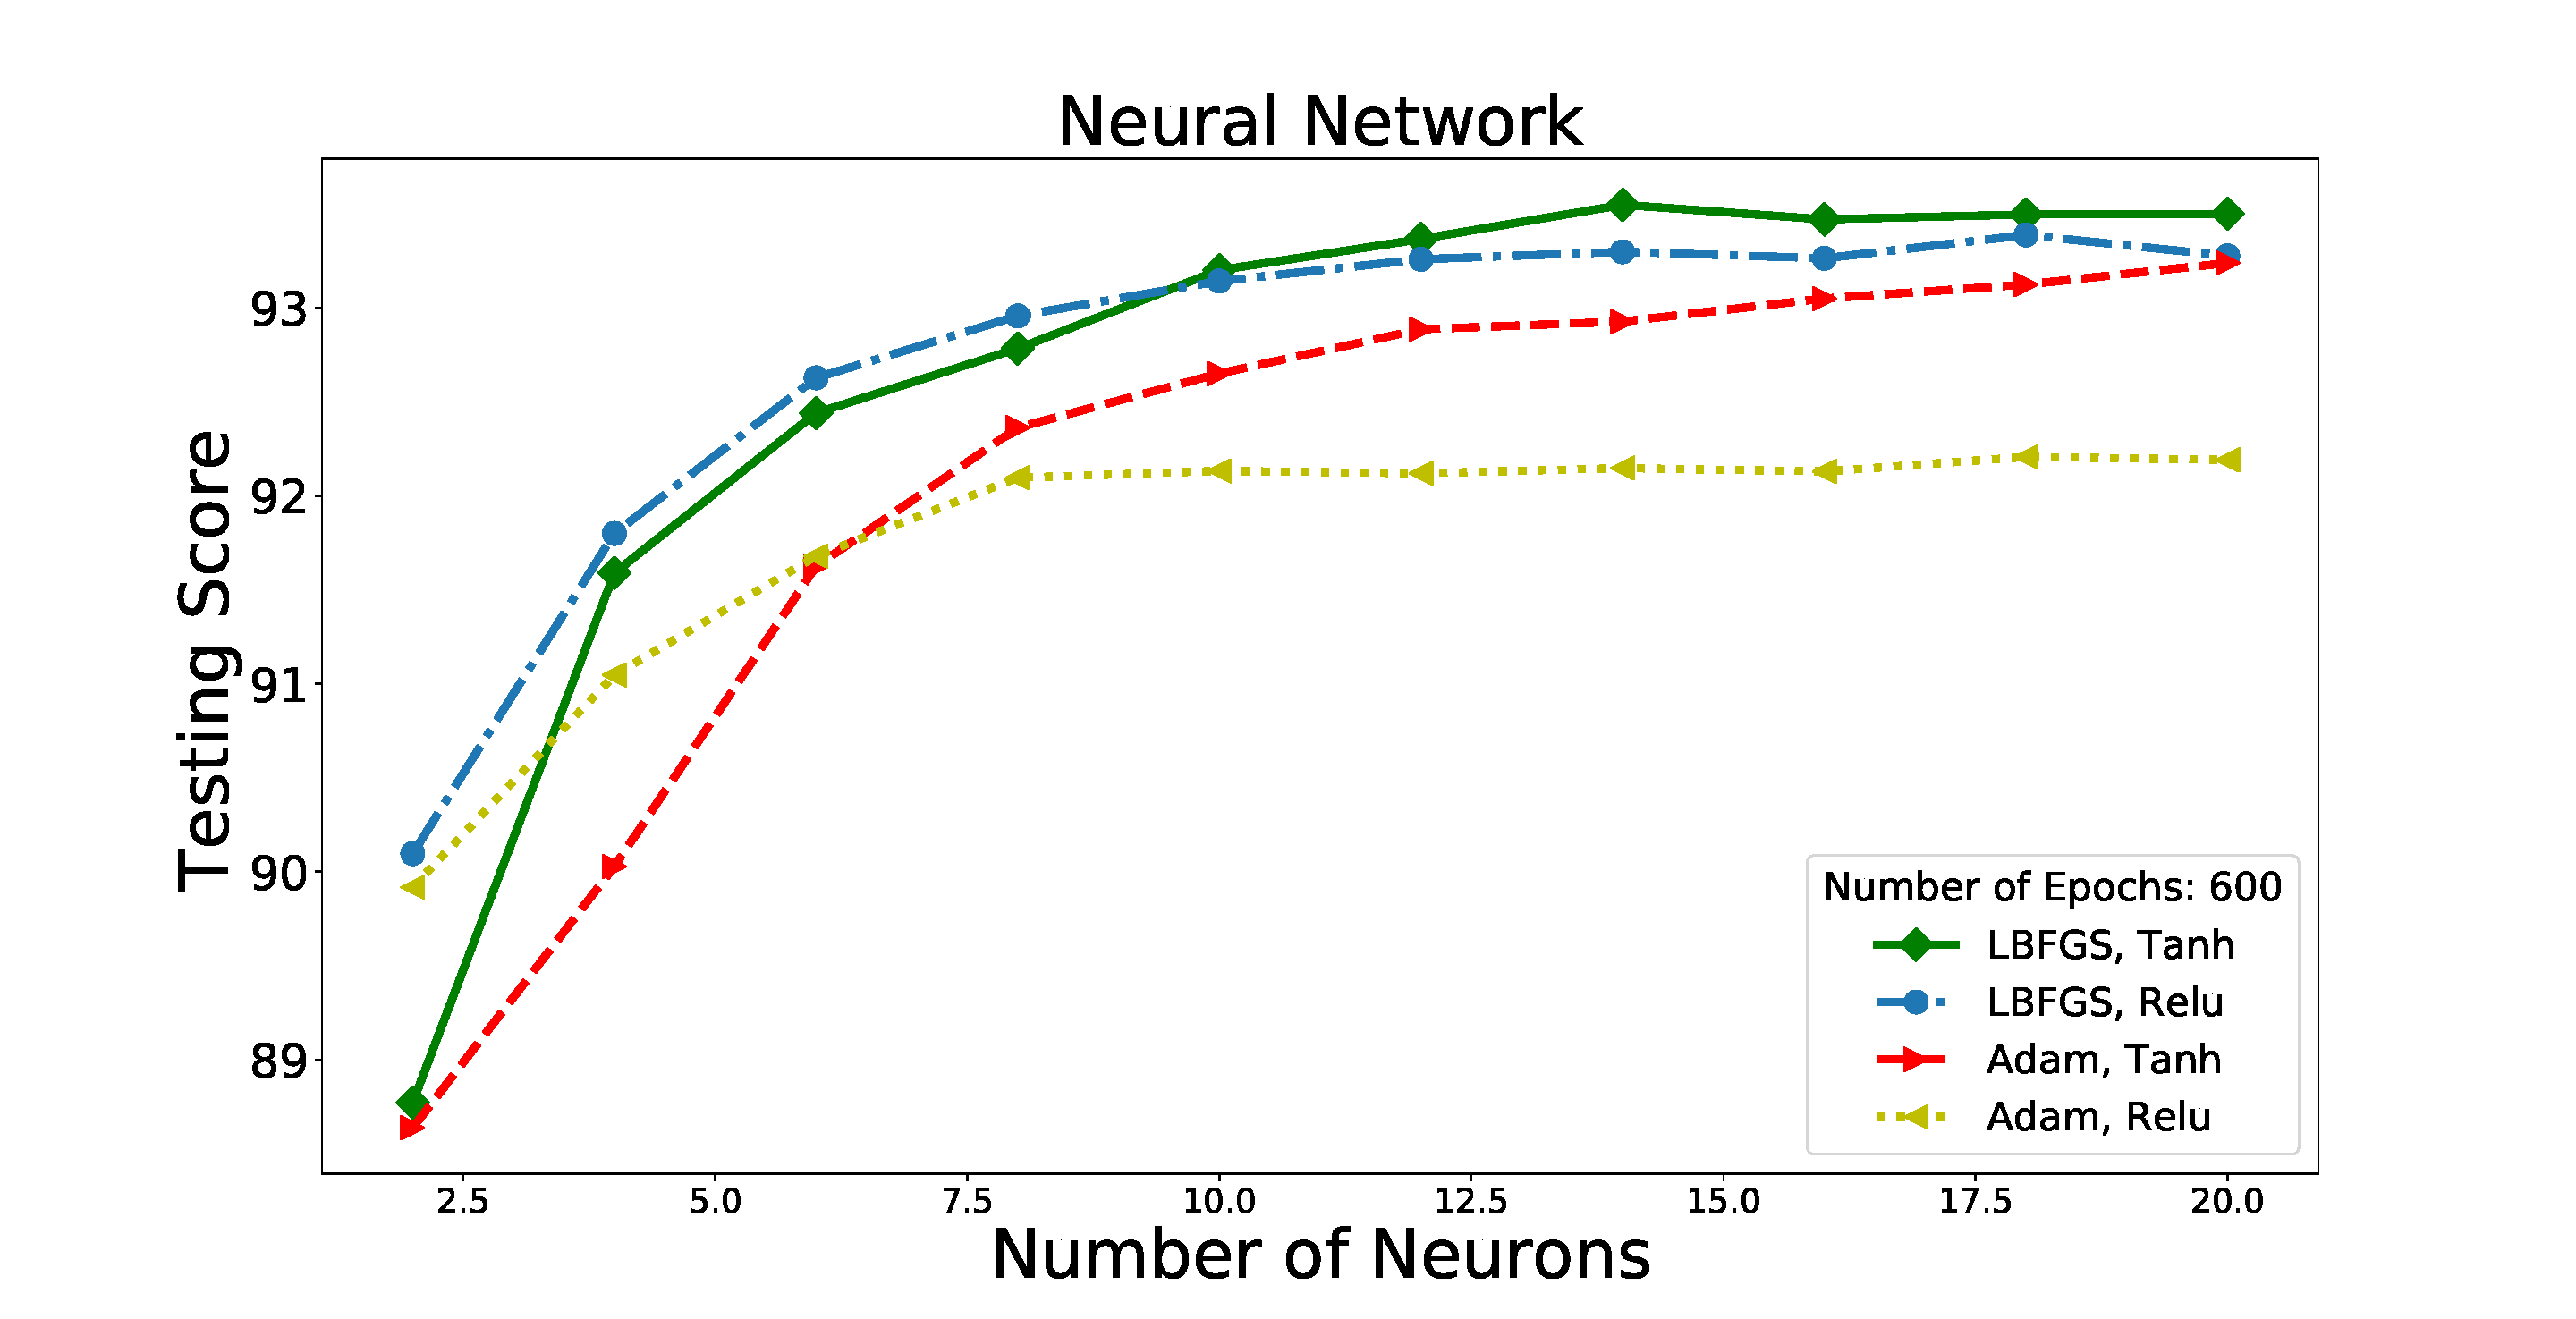
\includegraphics[width=0.5\textwidth]{plots/nn_neuron_train_multi.pdf}
\caption{Accuracy of the NN classification as a function of the number of epochs and of the number of neurons
 for the 3-class classification. 
 }
\label{fig:nets_multi}
\end{figure}


The dependence of accuracy on meta-parameters of the algorithms is shown in Figures \ref{fig:tree_multi} and \ref{fig:nets_multi}.
We see that for the tree-based algorithms, the optimal parameters are similar to the 2-class classification, i.e., 50 trees with depth 6 for RF and 100 trees with depth 2 for BDT 
provide close to optimal performance at a minimal cost in complexity (depth of the trees).
The main difference for NN and LR algorithms is that more steps are needed for convergence, especially in case of oversampling. 
In the following we use 600 epochs for NN and 500 iterations for LR instead of 300 epochs and 200 iterations respectively in the two-class case.
For NN, the accuracy stops increasing above about 10 neurons in the hidden layer (in the following we use 11 neurons for classification: the same as in the two-class case).
For oversampling, we use the oversampling factors $\sqrt{\frac{\text{\# AGN}}{\text{\# PSR}}}$ and $\sqrt{\frac{\text{\# AGN}}{\text{\# OTHER}}}$ for PSR and OTHER classes respectively (instead of $\frac{\text{\# AGN}}{\text{\# PSR}}$ and $\frac{\text{\# AGN}}{\text{\# OTHER}}$ oversampling factors in the 2-class case).
The reason for a smaller oversampling factors is to avoid overweighting the relatively small OTHER class.

\begin{figure}[h]
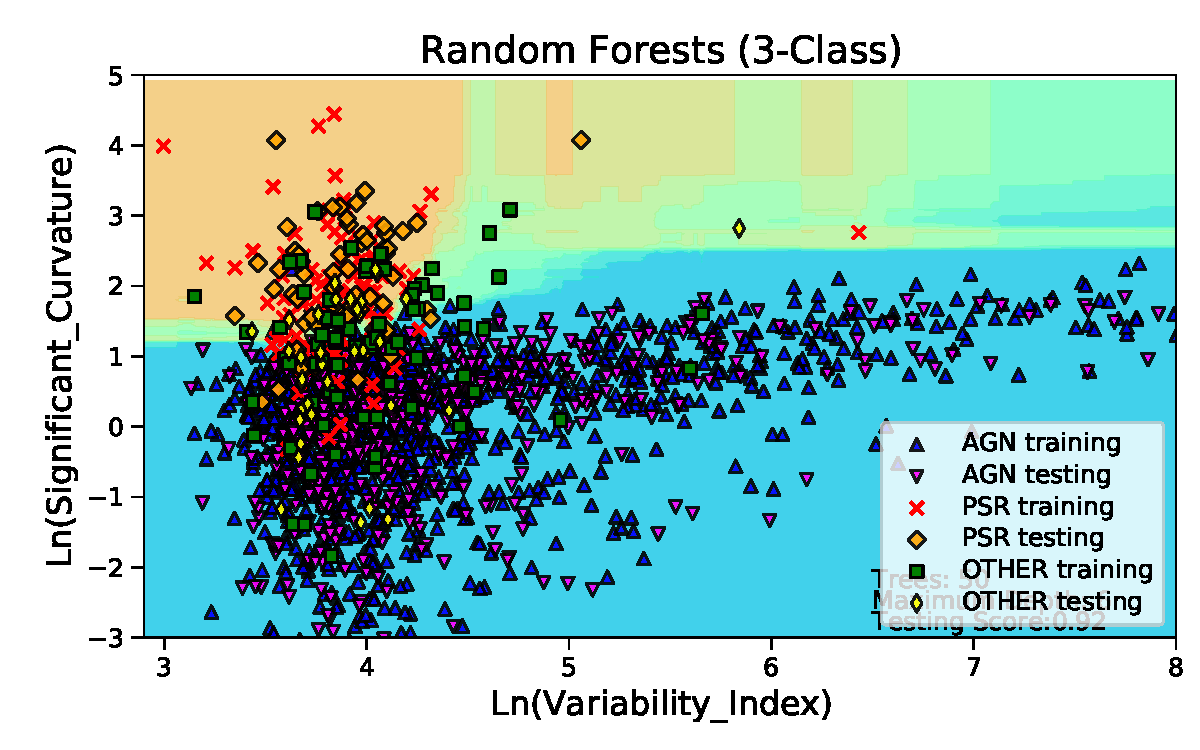
\includegraphics[width=0.46\textwidth]{plots/classification_domains/rf_50_6_3class.pdf}
\caption{Classification domains for RF in the 3-class classification.
}
\label{fig:RF_domains_3class}
\end{figure}

We show an example of domains in the 3-class case in Figure \ref{fig:RF_domains_3class}.
A class domain is determined by the class with the largest probability.
Since in the 3-class case there are two independent probabilities, which are difficult to show with a single color bar,
we present only the domains represented by three different colors: brown for PSR, green for OTHER, and blue for AGN classes.
The corresponding training and testing data are shown by red crosses and brown rotated squares for PSR, by green squares and yellow diamonds for OTHER,
and by blue and purple triangles for AGN classes.
The classification domains are averaged over 100 realizations of splitting the data into training and testing samples.
One of these splittings is shown on the figure.


The accuracies of our chosen models for classification of the 3FGL sources are presented in Table \ref{tab:selected_algs_multi}.
As in the 2-class case, the accuracies are averaged over 1000 realizations of splitting the data into training and testing samples.
We notice that accuracies presented in Table \ref{tab:selected_algs} are calculated relative to AGN and PSR classes only, if we take into account that all OTHER sources
are misclassified in this case, then the testing accuracy is reduced by about 5\% (the fraction of OTHER sources among associated sources in 3FGL),
while the accuracy of comparison with 4FGL-DR2 is reduced by about 10\% (there are 37 unassociated sources in 3FGL with OTHER class associations in 4FGL-DR2,
while there are in total 339 unassociated sources in 3FGL with associations in 4FGL-DR2).
Thus the testing accuracy of 93-94\% in Table \ref{tab:selected_algs_multi} provides at least a 1-2\% improvement over the accuracy in Table \ref{tab:selected_algs},
after taking into account the misclassification of OTHER sources in the 2-class case
and a similar improvement for the accuracy of classification of unassociated sources in 3FGL with 4FGL-DR2 associations.



\begin{table}[!h]
\hspace{-0.2cm}
\resizebox{0.47\textwidth}{!}{
    \tiny
  \centering
    \renewcommand{\tabcolsep}{0.4mm}
\renewcommand{\arraystretch}{1.6}

%\hspace{-3mm}
    \begin{tabular}{c c c c c c c}
    \hline
    \hline
    Algorithm&Parameters &  Testing\ &Std. Dev.& Comparison with \\
    & & Accuracy\ & & 4FGL-DR2 Accuracy \\
    \hline
    RF & 50 trees, max depth 6  & 93.96 & 0.85 & 85.00 \\
    RF\_O &   & 94.38 & 0.76 & 85.00 \\ 
    \hline
    BDT & 100 trees, max depth 2    &   93.72 & 0.83 & 83.24 \\
    BDT\_O &     &   93.83 & 0.80 & 85.29 \\
    \hline
    NN & 600 epochs, 11 neurons, LBFGS & 93.17 & 1.05 & 83.53 \\
    NN\_O &&  92.51 & 1.34 & 81.76 \\
    \hline
    LR & 500 iterations, LBFGS solver & 93.93 & 0.88 & 83.24 \\
    LR\_O &   & 93.01 & 0.96 & 83.24 \\
    \hline
    \end{tabular}}
    \vspace{2mm}
    \caption{Testing accuracy of the four selected algorithms for 3-class classification of 3FGL sources and comparison with associations in the 4FGL-DR2 catalog. 
    ``\_O'' denotes training with oversampling.}
    \label{tab:selected_algs_multi}
\end{table}



The 3-class classification of 4FGL-DR2 sources is performed similar to the 3-class classification of the 3FGL sources.
The differences are similar to the differences in the 2-class classification of 3FGL and 4FGL-DR2 sources:
we use 16 features (the same features as in the 2-class classification of 4FGL-DR2 sources in Section \ref{sec:4FGLprediction} but with GLON replaced by cos(GLON))
and we have 16 neurons in the hidden layer of the NN method. Furthermore, for Logistic Regression we use 1000 iterations instead of 500 as it gives better performance for oversampled cases.
The corresponding accuracies are reported in Table \ref{tab:selected_algs_4fgl_multi}.
In comparing the accuracies with the 2-class classification in Table \ref{tab:selected_algs2}, 
one has to take into account that there are 346 OTHER sources among 4116 associated sources in 4FGL-DR2, which is about 8.4\%.
Since all OTHER sources are ``misclassified'' by the 2-class classification, the 3-class classification provides an improvement of about 2-4\% compared to the 2-class classification.

\begin{table}[!h]
\hspace{-0.2cm}
%\resizebox{0.47\textwidth}{!}{
    \tiny
  \centering
    \renewcommand{\tabcolsep}{0.4mm}
\renewcommand{\arraystretch}{1.6}
    \begin{tabular}{c c c c c c}
    \hline
    \hline
    Algorithm&Parameters &  Testing&Std. Dev.\\
    & & Accuracy\ &  \\
    \hline
    RF & 50 trees, max depth 6  &92.91&0.66\\
    RF\_O &   &92.83&0.63 \\
    \hline
    BDT & 100 trees, max depth 2    &   92.51&0.67 \\
    BDT\_O &     &   92.27&0.67 \\
    \hline
    NN & 600 epochs, 16 neurons, LBFGS & 91.86&0.72\\
    NN\_O &  & 90.26&0.83\\
    \hline
    LR & 1000 iterations, LBFGS solver & 92.63&0.67 \\
    LR\_O &  &92.22&0.69\\
    \hline
     
    \end{tabular}%}
    \vspace{2mm}
    \caption{Testing accuracy of the four selected algorithms for the 3-class classification of 4FGL-DR2 sources. 
    ``\_O'' denotes training with oversampling.}
    \label{tab:selected_algs_4fgl_multi}
\end{table}


The numbers of unassociated sources classified by all 8 methods as AGNs, pulsars, and other sources for 3FGL and 4FGL-DR2 catalogs are presented in Table \ref{tab:prediction_2and3class} in the ``3-class'' rows.
For each algorithm the most probable class of the source is determined by the class with the largest probability.
Since there are three classes, the largest probability can have the value just above 1/3.
The ``Mixed'' column shows the number of sources with different classification results for different algorithms.

\begin{table}[!h]
%\resizebox{0.3\textwidth}{!}{
    %\tiny
  %\centering
 \renewcommand{\tabcolsep}{0.3mm}
\renewcommand{\arraystretch}{1.5}

    \begin{tabular}{l c c c c}
    \hline
    \hline
    4FGL-DR2 class & \multicolumn{4}{c}{3FGL prediction} \\
      &\ AGN &\ PSR &\ OTHER &\ MIXED \\
    \hline
    AGN & 238 & 2 &  1 & 17 \\ % 258
    PSR & 12 & 17 &  0 & 16 \\ % 45
    OTHER & 6 & 5 & 8 & 18 \\ % 37
    \hline
    \end{tabular}%}
    \vspace{0.2cm}
    \caption{Comparison of classes predicted for unassociated sources in the 3FGL catalog using 3-class classification
    with associations in the 4FGL-DR2 catalog. 
}
    \label{tab:3FGL_vs_4FGL_2class}
\end{table}


Classification of \Fermi-LAT 4FGL sources into three classes was considered earlier by, e.g., \cite{2021RAA....21...15Z}.
\cite{2021RAA....21...15Z} have primarily used a two-step classification procedure, where in the first step AGNs are separated from the rest of sources and in the second step the remaining sources are split into pulsars and other sources.
\cite{2021RAA....21...15Z} have also tested a simultaneous classification of sources into three classes (AGN, pulsars, other),
but the results were inconsistent for the two ML algorithms used by \cite{2021RAA....21...15Z} (RF and NN).
In particular, the number of OTHER sources predicted by NN was zero.
In our case, the predictions of various algorithms are relatively consistent with each other.
For example, in the 3FGL (4FGL-DR2) catalog all 8 methods classify 69 (271) unassociated sources as OTHER.
Also, 8 out of 37 unassociated 3FGL sources, which are associated to OTHER sources in 4FGL-DR2, are classified by all 8 algorithms as
OTHER (6 are classified as AGNs, 5 as PSRs, and 18 have mixed classification).

We also used the 3-class classification for a candidate list of most promising objects. We summed up the probabilities of all 8 methods for the three classes and chose the threshold of 7.0 for the column $\text{OTHER\_TOTAL}$. This is a stringent condition on the probability that a source belongs to the other class. Furthermore, we sub-selected the unassociated candidates in 4FGL-DR2 and have created our final candidate list of 30 sources based on 4FGL-DR2 features \footnote{6 of these sources also have a 3FGL name. 3 of these (4FGL J1312.6-6231c, 4FGL J1626.0-4917c, 4FGL J1631.7-4826c) are predicted to be OTHER based on 3FGL values, while the other 3 are predicted to be 'MIXED' sources.}. The maximum probability is $7.48\pm0.14$ for the source 4FGLJ1800.2-2403c. Out of these 30 sources only two have 0 flags in 4FGL, and only 8 have an association with the previous FGL catalogs (column name ASSOC\_FGL). Furthermore, we tried to find whether recent work could be found for some of these sources and used the Simbad database for this purpose. Out of the sources with Simbad entries the following 8 sources had extra associations (ordered according to probability of being OTHER source):
\begin{enumerate}
\item 4FGL J1800.2-2403c. The source with the greatest probability has no entry in Simbad. However, it is associated with the 1FGL source 1FGL J1800.5-2359c, which is also associated with the associated OTHER source 4FGL J1800.7-2355 of unk class and is in the region of the SNR W28 \citep{2020MNRAS.495.2909R}.
\item 4FGL J1842.7-0326: Associated with 3FGL J1843.7-0322 and found near the HESS source HESS J1843-033, next to the SNR G28.6-0.1 \citep{2018A&A...612A...1H}. This source was also the 67th source amongs 120 unassociated sources according to significance (>10) in the list of \citet{2016ApJ...820....8S} where the RF and LR methods predicted it to be a young pulsar based on the 2-class classification. In our 3FGL multi-class catalog, this source has a 'MIXED' prediction.
\item 4FGL J1626.0-4917c: In 3FGL as 3FGL J1626.2-4911. Part of the third Fermi catalog of hard sources as 3FHLJ1626.3-4915 \citep{2017ApJS..232...18A}. Associated with HESS J1626-490. It was also part of the 27 sources shortlisted by \citet{2020MNRAS.495.1093H} who used a machine learning technique to select sources for analysis from the 3FHL. Also has an 'OTHER' prediction based on 3FGL values.
\item 4FGL J1849.4-0117: In 3FGL as 3FGL J1849.5-0124c. In the region of Galactic mini starburst W43 studied by \citet{2020A&A...640A..60Y}. Has a 'MIXED' prediction for 3FGL values.
\item 4FGL J1109.4-6115e. In 3FGL as 3FGLJ1111.9-6038. Associated with the extended galactic source FGES J1109.4-6115 \citep{2017ApJ...843..139A}. Near the speculated SFR 4FGL J1115.1-6118 in there region of  Young Massive Stellar Cluster NGC 3603 \citep{2020ApJ...897..131S}. 'MIXED' prediction with 3FGL values.
\item 4FGL J1850.2-0201: Also in the region of the starburst W43 \citep{2020A&A...640A..60Y}.
\item 4FGL J1801.8-2358: Associated with HESS J1800-240A and 2FHL J1801.7-2358. Located south of the SNR W28 \citep{2020MNRAS.495.2909R}.
\item 4FGL J1855.8+0150: In the region of SNR W44 \citep{2020ApJ...896L..23P}.

\end{enumerate}
We have saved this candidate list with the rest of the catalogs. Furthermore, there are 6 PSR candidates in our multi-class classification with a probability sum $\text{PSR\_TOTAL}> 7.0$. These are the sources: 4FGL J1225.9+2951, 4FGL J2112.5-3043, 4FGL J1120.0-2204, 4FGL J0933.8-6232, 4FGL J0953.6-1509, 4FGL J1539.4-3323. All of these sources are also predicted to be pulsars as part of our 29 PSR sources mentioned in section 4 (using both 4FGL and 3FGL features). 2 of these are also present in the Parkes survey mentioned before.